\begin{enumerate}



\item Las plantas que poseen flores se originan por reproducción  sexual. En este proceso siempre intervienen dos componentes: uno masculino y otro femenino. Siguiendo el esquema   de la derecha que representa la fecundación vegetal en los momentos I y II, usted diría que este proceso ocurre exactamente cuándo: \label{bio-2}
\begin{center}
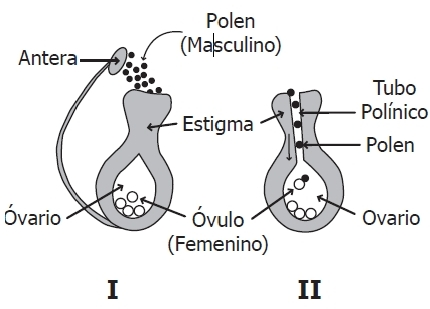
\includegraphics[width=0.45\textwidth]{bio_1.jpg} 
\end{center}
\begin{enumerate}[(A)]
\item El grano de polen se deposita sobre el estigma.
\item El polen se une con el óvulo en el ovario.
\item El óvulo madura y es el único componente que interviene.
\item El polen se une con el óvulo en el tubo polínico.
\end{enumerate}


%%%%%%%%%%%%%%%%%%%%%%%%%%%%
\newpage
\item La reproducción asexual se presenta    principalmente en tres modalidades. Cuando en la pared del progenitor se forma un brote o yema se desarrolla y se transforma en un nuevo individuo que se separa para vivir independientemente se conoce con el nombre de: \label{bio-1}
\begin{enumerate}[(A)]
\item Reproducción sexual 
\item Fecundación externa 
\item Gemación 
\item Regeneración 
\end{enumerate}
%%%%%%%%%%%%%%%%%%%%%%%%%%%%%%%%%%%%%%%%%%%%
\item En una especie de planta, el gen para flores rojas ($R$) es dominante sobre el gen para flores blancas ($r$). El siguiente cuadro de Punnett muestra el cruce entre una planta pura (homocigota) con flores rojas y una planta pura con flores blancas: \label{bio-3}\\[-1.1cm]
\begin{center}
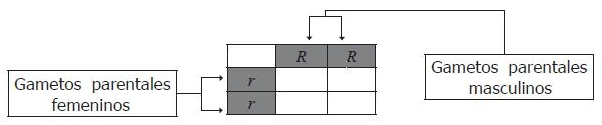
\includegraphics[width=0.45\textwidth]{bio_2.jpg} 
\end{center}
En el cuadro de Punnet las letras $R$ y $r$ simbolizan los alelos del gen para el color. Un alelo queda en cada gameto debido al proceso de 
\begin{enumerate}[(A)]
\item Meiosis.
\item Mitosis.
\item Fecundación.
\item Reproducción asexual.
\end{enumerate}
%%%%%%%%%%%%%%%%%%%%%%%%%%%%%%%%%%%%%
\item En los guisantes el gen que determina el color amarillo (A) domina sobre el que determina el color verde (a) que es recesivo. En el esquema  se representa: \label{bio-4}

\begin{center}
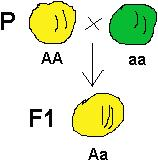
\includegraphics[width=0.35\textwidth]{bio_3.jpg} 
\end{center}
\begin{enumerate}[(A)]
\item La primera ley de Mendel.
\item La segunda ley de Mendel.
\item La tercera ley de Mendel.
\item Un cruce dihíbrido.
\end{enumerate}

%%%%%%%%%%%%%%%%%%%%%%%%%%%%%%%%%%%%%%%%%%%
\item Observa los siguientes dibujos: \label{bio-5}

\begin{center}
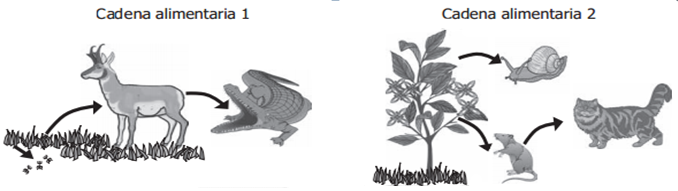
\includegraphics[width=0.5\textwidth]{bio_4} 
\end{center}

Según estas dos cadenas, ¿Cuales seres vivos ocupan el mismo nivel trófico?

\begin{enumerate}[(A)]
\item  as hormigas y el pasto.
\item El venado y el gato.
\item El cocodrilo y el gato.
\item El cocodrilo y el ratón.
\end{enumerate}


%%%%%%%%%%%%%%%%%%%%%%%%%%%%%%%%%%%%%%%%%%%%%%%%
\newpage
\item En una isla (A) se encuentra una especie de lagartijas conformadas por hembras. Por esta razón la reproducción es asexual y en consecuencia las hijas son una copia idéntica de la madre.  Por otro lado, en una isla cercana (B) hay otra especie de lagartijas con machos y hembras que se reproducen sexualmente.  La siguiente grafica representa la población de lagartijas en cada una de las islas:\label{bio-6}

Si una enfermedad comienza a provocar la muerte de las poblaciones de lagartijas en las islas ¿en cuál de ellas es más  probable que la población de lagartijas sobreviva?.


\begin{center}
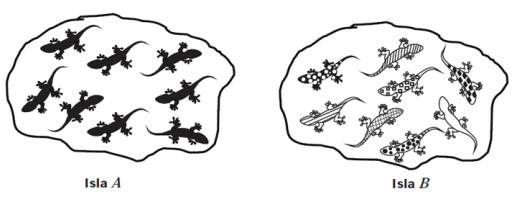
\includegraphics[width=0.45\textwidth]{bio_5.jpg} 
\end{center}
\begin{enumerate}[(A)]
\item En la isla A porque todas las lagartijas son genéticamente iguales.
\item En la isla A porque las hembras son más resistentes.
\item En la isla B porque la variabilidad genética de las lagartijas es alta. 
\item En la isla b porque las lagartijas macho son m\'as fuertes.
\end{enumerate}

%%%%%%%%%%%%%%%%%%%%%%%%%%%%%%%%%%%%%%%%%%%%%%%%%%%%%%%%%%%%5
\newpage
\subsubsection*{Responda las preguntas \ref{bio-7} y \ref{bio-8} de acuerdo con la siguiente información}
Una especie de mono presentaba alta tasa de predación debido a su poca agilidad para escapar de sus depredadores. En un momento de su historia evolutiva surgieron individuos con brazos más largos que lograron huir con más facilidad. En la actualidad la mayoría de los monos de dicha especie presentan brazos largos.


%%%%%%%%%%%%%%%%%%%%%%%%%%%%%%%%%%%%%%%%%%%%%5
\item  Según los principios de Darwin y analizando la evolución de dicha especie de monos se podría plantear que con mayor probabilidad: \label{bio-7}

\begin{enumerate}[(A)]
\item En una época determinada la característica de los brazos largos apareció simultáneamente en la mayoría de los individuos, los cuales al reproducirse heredaron esta característica a sus hijos.
\item El tamaño largo de los brazos se logró poco a poco y de manera individual a medida que los monos huían de sus depredadores, los actuales monos de brazos largos son producto de la ejercitación de los brazos.
\item El tamaño largo de los brazos fue una característica que apareció al azar, se heredó y afectó el éxito reproductivo de generación en generación hasta que la mayor parte de los individuos de esta especie tuvieron brazos largos.
\item Los brazos largos los obtuvieron algunos individuos al azar, característica que no se heredó por carecer de utilidad para la especie.
\end{enumerate}

%%%%%%%%%%%%%%%%%%%%%%%%%%%%%%%%%%%%%%%%%%%%%%%%%%%%%%%%%%%%%%%%%%%
\newpage
\item En la actualidad, esta especie de mono es exitosa en bosques húmedos tropicales. Debido a sus movimientos estos monos deben consumir diariamente gran cantidad de energía, por lo que requieren una dieta rica en calorías. De las siguientes, la dieta que mejor se acomodaría a los requerimientos de estos monos sería: \label{bio-8}

\begin{center}
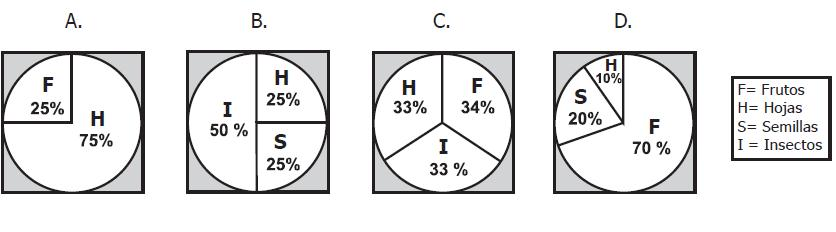
\includegraphics[width=0.45\textwidth]{bio_6.jpg} 
\end{center}


%%%%%%%%%%%%%%%%%%%%%%%%%%%%%%%%%%%%%%%%%%%%%%%%%%%%%%%%%%%%%%%%%%%
\item El siguiente dibujo muestra un experimento en el que se sembraron plantas en soluciones que contenían diferentes nutrientes. \label{bio-9}

\begin{center}
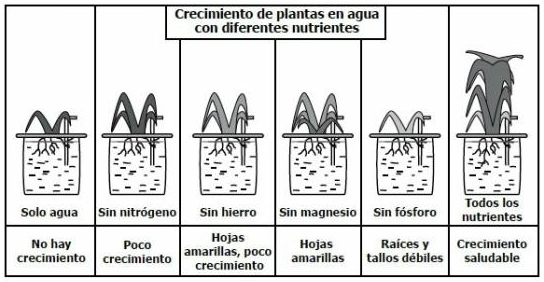
\includegraphics[width=0.45\textwidth]{bio_7.jpg} 
\end{center}

La pregunta que puede responderse con base en los resultados de este experimento es:

\begin{enumerate}[(A)]
\item ¿Cuál  es el efecto de cada nutriente en la absorción de agua en las plantas?
\item ¿Cuál  es el efecto de cada nutriente en el desarrollo de las plantas?
\item ¿Cuál  es el nivel mínimo de nutrientes en que una planta puede crecer?
\item ¿Cuál  eses el efecto del agua en la absorción de nutrientes en las plantas?
\end{enumerate}

%%%%%%%%%%%%%%%%%%%%%%%%%%%%%%%%%%%%%%%%%%%%%%%%%%%%%%%%%%%%%%%%%%%
\newpage
\item Los receptores sensosiales son parte del sistema nerviosdos de los animales y les permiten a estos percibir el ambiente.  Se metio un raton en un  cuarto oscuro donde habia un trozo de queso con olor agradable para el animal.  ¿Cuáles fueron los receptores sensoriales que uso el ratón para llegar al queso? \label{bio-10}

\begin{enumerate}[(A)]
\item Quimiorreceptores y termorreceptores.
\item Mecanorreceptores y receptores de dolor.
\item Termorreceptores y fotorreceptores.
\item Quimiorreceptores y mecanorreceptores.
\end{enumerate}


\subsubsection*{Las preguntas \ref{bio-11} a la \ref{bio-13}  se contestan teniendo en cuenta la siguiente lectura}

Las enfermedades de transmisión sexual (ETS), causadas por virus, bacterias, protistas o artrópodos que infectan los órganos sexuales o el aparato reproductor representan un serio y creciente problema de salud en todo el mundo. La Organización Mundial de la Salud calcula que hay 250 millones de casos nuevos de ETS cada año. Como su nombre lo dice, estas enfermedades se transmiten ya sea exclusiva o principalmente a través del contacto sexual. 


Algunas de las enfermedades más comunes de este tipo son: 
Infecciones bacterianas, la gonorrea, una infección del aparato genital y urinario, es una de las más comunes de todas las enfermedades infecciosas y se calcula que infecta a por lo menos dos millones de personas cada año. 

La bacteria causante, la cual no puede sobrevivir fuera del cuerpo, se transmite casi exclusivamente por contacto íntimo. Penetra las membranas limitantes de la uretra, ano, cérvix, útero, oviductos y garganta. En los hombres, la inflamación de la uretra da como resultado la salida de pus por el pene y una micción dolorosa, Aproximadamente el 10\% de los hombres infectados y 50\% de las mujeres infectadas tienen síntomas ligeros o ausentes y, por tanto, no buscan tratamiento. Se convierten en portadores quienes pueden diseminar fácilmente la enfermedad. La gonorrea puede ocasionar infertilidad al bloquear los oviductos con tejido cicatrizante. El tratamiento con penicilina en un principio fue muy satisfactorio, pero las cepas resistentes ahora requieren el uso de otros antibióticos. Los niños nacidos de madres infectadas pueden adquirir la bacteria durante el parto. La bacteria ataca a los ojos de los recién nacidos y en alguna ocasión representó una causa importante de ceguera. Hoy en día, a la mayoría de los nacidos se les administran inmediatamente gotas con antibiótico para matar esta bacteria. 

%%%%%%%%%%%%%%%%%%%%%%%%%%%%%%%%%%%%%%%%%%%%%%%%%%%%%%%%%%%%%%%%%%%
\item La gonorrea, una infección del aparato genital y urinario, es una de las más comunes de todas las enfermedades infecciosas, en su etapa inicial: \label{bio-11}

\begin{enumerate}[(A)]
\item Afecta los ojos de los recién nacidos y en alguna ocasión representó una causa importante de ceguera. 
\item Penetra las membranas limitantes de la uretra, ano, cérvix, útero, oviductos y garganta.
\item Puede ocasionar infertilidad al bloquear los oviductos con tejido cicatrizar. 
\item Los niños nacidos de madres infectadas pueden adquirir la bacteria durante el parto. 
\end{enumerate}


%%%%%%%%%%%%%%%%%%%%%%%%%%%%%%%%%%%%%%%%%%%%%%%%%%%%%%%%%%%%%%%%%%%
\item Para combatir la gonorrea se utiliza: \label{bio-12}

\begin{enumerate}[(A)]
\item Penicilina y analgésicos. 
\item Penicilina y barbitúricos. 
\item Penicilina y antibióticos. 
\item Penicilina y calmantes. 
\end{enumerate}

%%%%%%%%%%%%%%%%%%%%%%%%%%%%%%%%%%%%%%%%%%%%%%%%%%%%%%%%%%%%%%%%%%%
\item  Las enfermedades de transmisión\\ sexual (ETS), son causadas por:\label{bio-13}

\begin{enumerate}[(A)]
\item Vírus, leveduras, protistas o\\ garrapatas. 
\item Vírus, bactérias, protistas o\\ artrópodos. 
\item Vírus, bactérias, nematódeos o\\ artrópodos. 
\item Vírus, hongos, protistas o\\ garrapatas.
\end{enumerate}

%%%%%%%%%%%%%%%%%%%%%%%%%%%%%%%%%%%%%%%%%%%%%%%%%%%%%%%%%%%%%%%%%%%
\item En la figura se muestra  la localización  del gen que produce una proteína en humanos. Cuándo este gen muta (figura    derecha), produce una proteína diferente de la proteína normal. Lo que determina la proteína que produce el gen es:  \label{bio-14}
\begin{center}
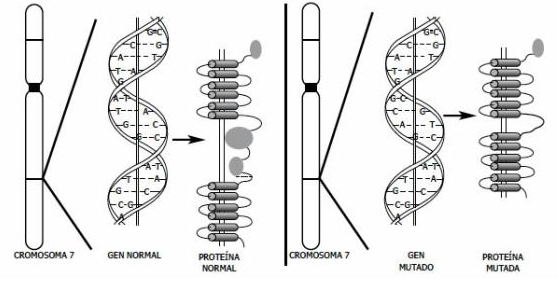
\includegraphics[width=0.45\textwidth]{bio_8.jpg} 
\end{center}
\begin{enumerate}[(A)]
\item El  cromosoma  al  que pertenece  el gen.
\item La secuencia de  nucleótidos  que posee.
\item Su  localización dentro   del cromosoma.
\item La  configuración  helicoidea el ADN.	
\end{enumerate}


%%%%%%%%%%%%%%%%%%%%%%%%%%%%%%%%%%%%%%%%%%%%%%%%%%%%%%%%%%%%%%%%%%%
\newpage
\item Unos   investigadores  evaluaron  la relación ecológica de los insectos consumidores de néctar y una planta de interés comercial.  Como resultado  reportaron los datos  en las siguientes gráficas \label{bio-15}
\begin{center}
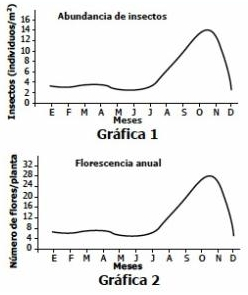
\includegraphics[width=0.45\textwidth]{bio_9.jpg} 
\end{center}
A partir   de las  gráficas.  Una de las  relaciones  que  se puede  proponer  entre los insectos y planta  es   que los insectos:
\begin{enumerate}[(A)]
\item Dispersan los frutos de la planta.
\item Se alimenta de las hojas de la planta.
\item Polinizan la  planta.
\item Nutren la   planta.
\end{enumerate}


%%%%%%%%%%%%%%%%%%%%%%%%%%%%%%%%%%%%%%%%%%%%%%%%%%%%%%%%%%%%%%%%%%%
\newpage
\item Los  antibióticos   son sustancias  químicas  que impiden  el  crecimiento de   las  bacterias.  Por  sus  características, los  antibióticos  se   utilizan   para tratar   infecciones.  Sin  embargo, algunos  microrganismos  pueden   ser  resistentes  y trasmitirlo   a  su descendencia.  Una  forma  de evitar  la  resistencia a los antibióticos   por parte   de los  microorganismos   es: \label{bio-16}


\begin{enumerate}[(A)]
\item Utilizar  otros  medicamentos  regulares.
\item Seguir  el tratamiento  recomendado para  el antibiótico.
\item No utilizar  antibiótico.
\item Evitar  el contacto  con las bacterias resistentes.
\end{enumerate}


%%%%%%%%%%%%%%%%%%%%%%%%%%%%%%%%%%%%%%%%%%%%%%%%%%%%%%%%%%%%%%%%%%%
\item  Observe el siguiente  modelo  del flujo   de la energía  en un ecosistema. \label{bio-18}
\begin{center}
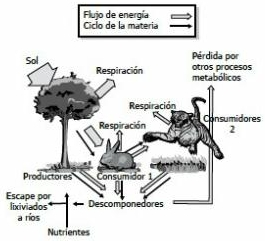
\includegraphics[width=0.45\textwidth]{bio_11.jpg} 
\end{center}
Según  el modelo se puede  concluir   que  este ecosistema es  un sistema  abierto ¿por qué?
\begin{enumerate}[(A)]
\item Los seres vivos usan el alimento para transformarlo en energía.
\item Varios  nutrientes  pueden salir por  lixiviados  a otros ecosistemas.
\item Los descomponedores  trasforman  los desechos   en nutrientes  para las plantas.
\item La energía fluye  a través  de los niveles    tróficos.
\end{enumerate}
%%%%%%%%%%%%%%%%%%%%%%%%%%%%%%%%%%%%%%%%%%%%%%%%%%%%%%%%%%%%%%%%%%%
\item Las  abejas  tienen un  completo   sistema   de   dos  pares  de  alas   unidas    entre  sí    que  se mueven  al tiempo,   como se  observa  en el siguiente  dibujo. \label{bio-17}
\begin{center}
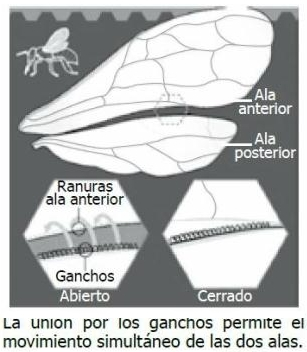
\includegraphics[width=0.45\textwidth]{bio_10.jpg} 
\end{center}
Para  lograr  el vuelo rápido las  abejas  necesitan:
\begin{enumerate}[(A)]
\item Músculos  para mover  las  alas.
\item Exoesqueleto  articulado  que permita flexibilidad de durante  el  vuelo.
\item Hormonas para estimular el movimiento.
\item  Venas en las alas que  le den rigidez.
\end{enumerate}



%%%%%%%%%%%%%%%%%%%%%%%%%%%%%%%%%%%%%%%%%%%%%%%%%%%%%%%%%%%%%%%%%%%
\newpage
\item El dióxido de carbono (CO2) se reconoce  como el gas  más  importante junto al  metano  y los   hidroflurocarbonos  en el calentamiento global. La actividad  humana  ha llevado  al    incremento de  este gas en la atmósfera, aunque las plantas y las algas fijan este gas  disminuyendo su  concentración.  Se determinó  el aporte del CO2  a la atmósfera en 4  zonas y los resultados se mostraron  en la siguiente gráfica. \label{bio-19}


\begin{center}
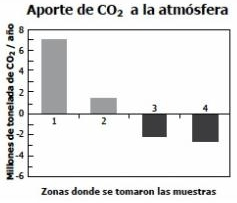
\includegraphics[width=0.45\textwidth]{bio_12.jpg} 
\end{center}
Según los resultados anteriores,  a  que corresponde   cada  una de las zonas en la gráfica: 

\begin{enumerate}[(A)]
\item Zona 1: Océano.   Zona 2: Bosque. Zona 3: Rular.    Zona 4: Fabricas.
\item Zona 1: Bosque.   Zona 2: Rural.  Zona 3: Fabricas. Zona 4: Océano.
\item Zona 1: Fabricas. Zona 2: Rural.  Zona 3: Bosque.   Zona 4: Oceano.
\item Zona 1: Bosque.   Zona 2: Océano. Zona 3: Rural.    Zona 4: Fabric.
\end{enumerate}


%%%%%%%%%%%%%%%%%%%%%%%%%%%%%%%%%%%%%%%%%%%%%%%%%%%%%%%%%%%%%%%%%%%
\newpage
\item Entre  los  años  de  1845 y 1852, todos  los  cultivos  de papa  de  la isla de  Irlanda  fueron   destruidos por  una enfermedad  producida por un  hongo. Dos factores  contribuyen  a la  alta  dispersión de  la  enfermedad: \label{bio-20}
(1)en Irlanda  se cultivaba únicamente una variedad de papa y (2) los  cultivos  de papa  se  encontraban aislados del resto de  mundo, por lo  cual se producía únicamente entre sí.
Desde un punto de  vista genético estos  2  factores contribuyeron  a la dispersión de la enfermedad por qué:
\begin{enumerate}[(A)]
\item Se  redujo  la variedad  genética de los cultivos  de papa  haciéndolos susceptibles a la epidemia.
\item Produjeron una alta  variedad  genética  generando plantas  de  papas  muy  diferentes entre  si  y  susceptibles  a la epidemia.
\item El genoma     del  hongo  se incorporó rápidamente  al  ADN  de las papas y la enfermedad  se trasmitió genéticamente.
\item Ocasiones  un   aumento  en  el número  de  cromosomas  de  las  papas  cultivadas, haciéndolas    susceptibles  a   la  epidemia.
\end{enumerate}

%%%%%%%%%%%%%%%%%%%%%%%%%%%%%%%%%%%%%%%%%%%%%%%%%%%%%%%%%%%%%%%%%%%
\item Observa la  figura \label{bio-22}\\[-1.1cm]
\begin{center}
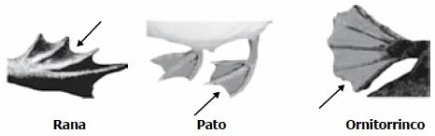
\includegraphics[width=0.45\textwidth]{bio_13.jpg} 
\end{center}
Las  flechas    en la figura    muestran  la membrana   interdactilar  que se encuentra en las extremidades de animales  como ranas  acuáticas patos    y ornitorrincos. Está membrana  es común   en estos  animales ¿por qué?
\begin{enumerate}[(A)]
\item Descienden   de  un ancestro común  cercano.
\item Evolucionaron al mismo tiempo.
\item Se desplazan en medios acuáticos.
\item Les sirve para agarrar la presa.
\end{enumerate}
%%%%%%%%%%%%%%%%%%%%%%%%%%%%%%%%%%%%%%%%%%%%%%%%%%%%%%%%%%%%%%%%%%%
\item El  alcohol   es  una  sustancia  que  puede generar  dependencia en  las  personas  que  lo  consumen, inhibe  la  producción  de glóbulos blancos, genera un deterioro  de las mucosas  del   sistema  digestivo , incrementa la  actividad  cardiaca  y  altera la acción  de  algunos  neurotransmisores. \label{bio-21}

De  acuerdo  con  lo  anterior,  cuál  de las  siguientes  alteraciones en  la  salud , estaría  relacionada  con el consumo  excesivo  de  alcohol.

\begin{enumerate}[(A)]
\item Ser  propenso a contraer  infecciones  bacterianas o  virales.
\item Tener  una baja producción  de  gástricos  en el estómago.
\item Aumentar  el  estado  de  alerta  y la  velocidad  de los  reflejos.
\item Reducir significativamente  la  presión   arterial.
\end{enumerate}

%%%%%%%%%%%%%%%%%%%%%%%%%%%%%%%%%%%%%%%%%%%%%%%%%%%%%%%%%%%%%%%%%%%
\item Observe la siguiente red alimenticia que existe en un ecosistema. Teniendo en cuenta las relaciones establecidas en la anterior red alimentaria, ¿Qué se espera que suceda con la población de sapos si todos los peces pequeños se extinguen? ¿Por qué? \label{bio-25}
\begin{center}
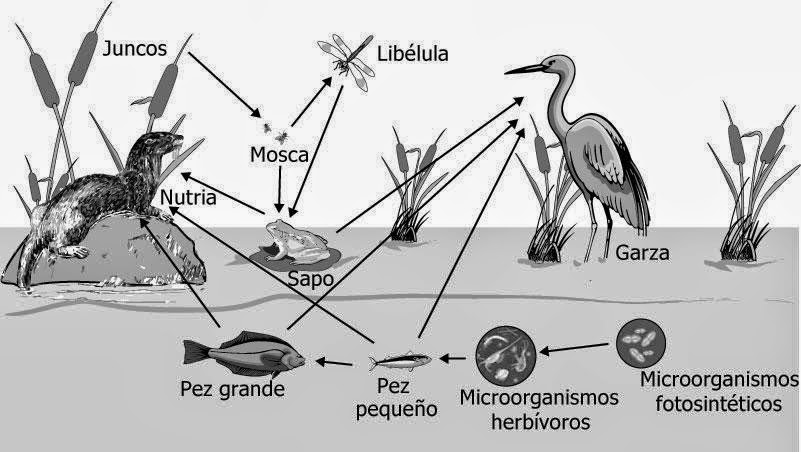
\includegraphics[width=0.45\textwidth]{bio_14.jpg} 
\end{center}
Para responder esta pregunta lo debe hacer en las líneas siguientes sin salirse del recuadro, debe ser clara y concisa  \hrulefill\\
\_\hrulefill\\
\_\hrulefill\\
\_\hrulefill\hrulefill\\
\_\hrulefill

%%%%%%%%%%%%%%%%%%%%%%%%%%%%%%%%%%%55
\newpage
\item La  leshmaneasis  es una  enfermedad   tropical   cuyos   síntomas     característicos   son ulceras cutáneas   e inflamación del  hígado  y del bazo.  Se  trasmite  principalmente   por la picadura   de  insectos  hematófagos    que  inyectan en la victima  un   protozoario  del  genero Leishmania, aunque también  puede trasmitirse por transfusiones   de  sangre infectadas    o con  congénitamente.  A partir  de esta información sobre la leishmaniasis  ¿Cuál de las  siguientes preguntas  puede resolverse      en una investigación de ciencias naturales?  \label{bio-23}       


\begin{enumerate}[(A)]
\item ¿Qué   ideas   y  concepciones  sobre el  ciclo de  vida de los  insectos hematófagos tiene las culturas   de los   países   afectados   por leishmaneasis?
\item ¿Cómo fluye  la presencia  de leishmaniasis   en el ingreso  per cápita  de los  países  de la región   ecuatorial?
\item ¿Por qué se inflama el hígado  y el bazo   de las personas  que han  sido infectadas con Leishmania?
\item ¿Qué políticas  deben    adoptarse    para l  asignación   de  recursos   para el control  de la enfermedad?
\end{enumerate}


%%%%%%%%%%%%%%%%%%%%%%%%%%%%%%%%%%%%%%%%%%%%%%%%%%%%%%%%%%%%%%%%%%%
\newpage
\item Durante la fotosíntesis, los estomas en las hojas permanecen abiertos  el tiempo suficiente para captar dióxido de carbono, lo que a su vez genera  una pérdida de agua por transpiración.  Los espacios que deja el agua transpirada tienen que ocuparse nuevamente  por moléculas de agua nueva, que ascienden a las hojas desde las raíces a través del xilema. Según esta información, se puede afirmar que los estomas son importantes en el proceso de nutrición de las plantas, porque: \label{bio-24}

\begin{enumerate}[(A)]
\item Son células especializadas en la absorción de sales minerales.
\item Por ellos ingresan sales que se distribuyen a toda la planta a través del xilema.
\item Cuando están abiertos permiten que el agua suba con iones para las células.
\item Permiten el flujo de sabia elaborada por el xilema.  
\end{enumerate}


%%%%%%%%%%%%%%%%%%%%%%%%%%%%%%%%%%%%%%%%%%%%%%%%%%%%%%%%%%%%%%%%%%%



%%%%%%%%%%%%%%%%%%%%%%%%%%%%%
\subsubsection*{Responda las preguntas \ref{bio-26} y \ref{bio-27} a partir de la  siguiente lectura}


\noindent Las bacterias son células procariotas sin núcleo definido en su interior. Su tamaño es unas diez veces inferior  de las células eucariotas. En su estructura podemos observar los siguientes componentes:\\
La pared bacteriana es una envoltura rígida y permeable, que da forma a las células bacterianas está rodeada por la membrana plasmática. Existen dos tipos de pared: Gram positiva y Gram negativa. La pared Gram positiva es monoestraficada, está formada por una capa basal de peptidoglucanos (mureína), a la cual se asocian polisacáridos, ácidos teicoicos y proteínas. La pared Gram negativa es biestratificada, con una capa basal de peptidoglucanos rodeada de una bicapa lipídica que además contiene fosfolípidos, polisacáridos y proteínas.\\

La membrana plasmática es una bicapa lipídica con proteínas, similar a la de las células eucariotas, pero más fluida. Mesosomas: la membrana presenta invaginaciones hacia el interior, en esta zona se encuentran las enzimas responsables de la respiración celular.  En el plasma del interior de las bacterias se encuentran los ribosomas que son más pequeños que los de las células eucariotas. Su función es la síntesis de proteínas. El cromosoma bacteriano es una molécula de ADN circular de doble cadena asociado con unas pocas proteínas que está anclado en un punto de la membrana plasmática.  Algunas bacterias tienen flagelos que sirven para el movimiento, otras tienen fimbrias o pelos  que sirven para adherirse a superficies.\\

Formas de nutrición en función de la fuente de carbono que utilicen las bacterias se dividen en:\\

\textbf{Autótrofas:} utilizan el CO2 como fuente de carbono para construir a partir de él todas sus biomoléculas orgánicas.\\

\textbf{Heterótrofas:} utilizan el carbono de moléculas orgánicas ya elaboradas por otros seres vivos.\\

Según la fuente de energía que utilizan, las bacterias pueden ser:\\

\textbf{Fotótrofas o fotosintéticas:} utilizan como fuente de energía la luz solar.\\

\textbf{Quimiótrofas o quimiosintéticas:} utilizan la energía liberada en las reacciones químicas exotérmicas, reacciones de óxido-reducción.


%%%%%%%%%%%%%%%%%%%%5
\newpage
\item Son componentes importantes de la estructura de una bacteria:\label{bio-26}


\begin{enumerate}[(A)]
\item Cílios, pelos, núcleo, ribosomas.
\item Pared, La membrana plasmática, el plasma, ADN.
\item Gram positiva y Gram negativa, ácidos teicoicos y proteínas.
\item Bicapa lipídica, fosfolípidos, polisacáridos y proteínas.
\end{enumerate}


%%%%%%%%%%%%%%%%%%%%%%%%%%%%%
\newpage
\item En relación a la forma de nutrición de las bacterias es correcto afirmar: \label{bio-27}


\begin{enumerate}[(A)]
\item Las bacterias autótrofas y heterótrofas utilizan el alimento presente en la atmósfera.
\item  Las bacterias Fotótrofas o fotosintéticas,  utilizan como fuente de energía el agua.
\item  Quimiótrofas o quimiosintéticas: utilizan la energía liberada en las reacciones químicas      exotérmicas, reacciones de óxido-reducción.
\item  Las bacterias son descomponedoras.
\end{enumerate}

%%%%%%%%%%%%%%%%%%%%%%%%%%%%%
\end{enumerate}
%%%%%%%%%%%%%%%%%%%%%%%%%%%%%